\section{投影相机模型}\label{sec:投影相机模型}

三维计算机图形学中的一个基本问题是{\itshape 3D视见问题}:
如何将三维场景投影到二维图像上进行显示。
大多数经典方法都可以用$4\times4$的\keyindex{投影变换}{projective transformation}{transformation变换}矩阵来表达。
因此,我们将引入一个投影矩阵相机类\refvar{ProjectiveCamera}{},
然后在此基础上定义两个相机模型。
第一个实现了\keyindex{正交投影}{orthographic projection}{projection投影},
另一个实现了\keyindex{透视投影}{perspective projection}{projection投影}——
两种经典且广泛使用的\keyindex{投影}{projection}{}。
\begin{lstlisting}
`\initcode{Camera Declarations}{+=}\lastcode{CameraDeclarations}`
class `\initvar{ProjectiveCamera}{}` : public `\refvar{Camera}{}` {
public:
    `\refcode{ProjectiveCamera Public Methods}{}`
protected:
    `\refcode{ProjectiveCamera Protected Data}{}`
};
\end{lstlisting}

还有三个坐标系(总结于\reffig{6.1}中)对定义和讨论投影相机很有用。
\begin{itemize}
    \item \keyindex{屏幕空间}{screen space}{}:
          屏幕空间定义在胶片平面上。相机将相机空间中的物体投影到胶片平面上;
          \keyindex{屏幕窗口}{screen window}{}内的部分在生成的图像中是可见的。
          屏幕空间的深度$z$值从0变到1,分别对应近处和远处截平面的点。
          注意,虽然这称为“屏幕”空间,但它仍然是一个三维坐标系,因为$z$值是有意义的。
    \item \keyindex{规范化设备坐标}{normalized device coordinate}{}(NDC){\sffamily 空间}:
          这是被渲染的实际图像的坐标系。对于$x$和$y$,该空间范围从$(0,0)$变到$(1,1)$,
          其中$(0,0)$是图像的左上角。深度值与屏幕空间中的相同,线性变换将屏幕空间转换为NDC空间。
    \item \keyindex{栅格空间}{raster space}{}\sidenote{译者注:也称光栅空间。}:
          这与NDC空间几乎相同,除了$x$和$y$坐标从$(0,0)$变到(resolution.x, resolution.y)
          \sidenote{译者注:resolution指分辨率。}。
\end{itemize}

投影相机用$4\times4$矩阵在所有这些空间之间进行转换,
但具有特殊成像特性的相机不必用矩阵表示所有这些转换。
\begin{figure}[htbp]
    \centering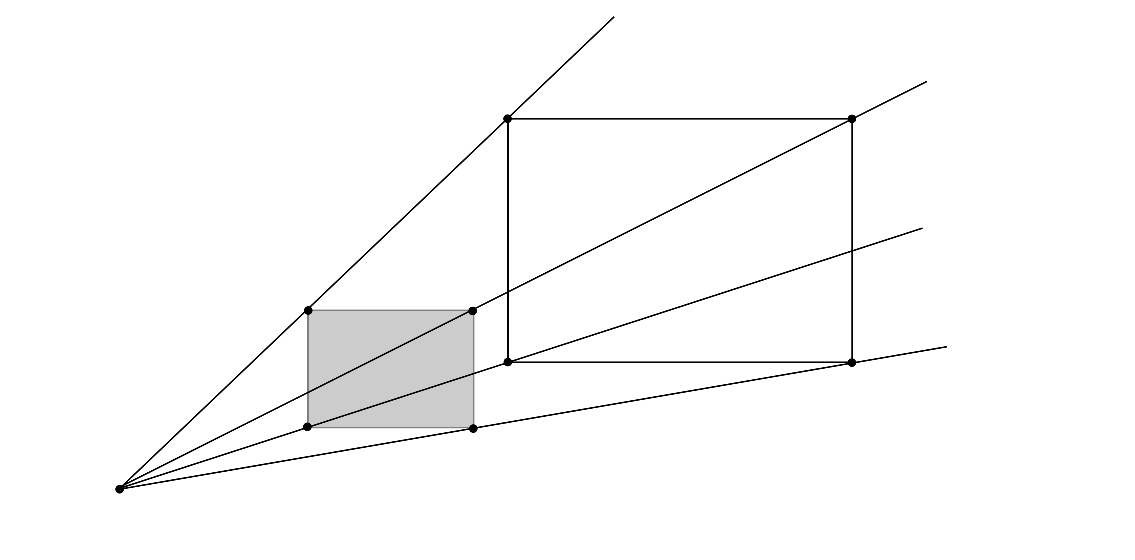
\includegraphics[width=0.75\linewidth]{chap06/Cameracoordinatespaces.eps}
    \put(-280,0){\small 相机空间:$(0,0,0)$}
    \put(-270,60){\small NDC:$(0,0,0)$}
    \put(-220,110){\small NDC:$(0,0,1)$}
    \put(-160,20){\small $z=\text{near}$}
    \put(-160,10){\small NDC:$(1,1,0)$}
    \put(-160,0){\small 栅格:$(\text{res}.x,\text{res}.y,0)$}
    \put(-70,35){\small $z=\text{far}$}
    \put(-70,25){\small NDC:$(1,1,1)$}
    \put(-70,15){\small 栅格:$(\text{res}.x,\text{res}.y,1)$}
    \caption{几个与相机相关的坐标空间常用于简化\protect\refvar{Camera}{}的实现。
        相机类持有它们之间的变换。世界空间中的场景物体由相机查看,它位于相机空间原点,并指向$+z$轴。
        近处和远处平面之间的物体被投影到相机空间中的胶片平面$z=\text{near}$上。
        胶片平面在栅格空间中$z=0$处,其中$x$和$y$范围从$(0,0)$变到(resolution.x, resolution.y)。
        规范化设备坐标(NDC)空间将栅格空间归一化,因此$x$和$y$范围从$(0,0)$变到$(1,1)$。}
    \label{fig:6.1}
\end{figure}

除了基类\refvar{Camera}{}要求的参数外,\refvar{ProjectiveCamera}{}还接收投影变换矩阵、
图像的屏幕空间范围以及与景深有关的额外参数。
\keyindex{景深}{depth of field}{}将在本节末尾介绍和实现,
它模拟了真实透镜系统中出现的失焦物体的模糊性。
\begin{lstlisting}
`\initcode{ProjectiveCamera Public Methods}{=}`
`\refvar{ProjectiveCamera}{}`(const `\refvar{AnimatedTransform}{}` &CameraToWorld, 
        const `\refvar{Transform}{}` &CameraToScreen, const `\refvar{Bounds2f}{}` &screenWindow,
        `\refvar{Float}{}` shutterOpen, `\refvar{Float}{}` shutterClose, `\refvar{Float}{}` lensr, `\refvar{Float}{}` focald,
        `\refvar{Film}{}` *film, const `\refvar{Medium}{}` *medium)
    : `\refvar{Camera}{}`(CameraToWorld, shutterOpen, shutterClose, film, medium),
      `\refvar{CameraToScreen}{}`(CameraToScreen) {
    `\refcode{Initialize depth of field parameters}{}`
    `\refcode{Compute projective camera transformations}{}`
}
\end{lstlisting}

\refvar{ProjectiveCamera}{}的实现将投影变换传递给这里展示的基类构造函数。
该变换给出了相机到屏幕的投影;
由此,构造函数能轻松算出从栅格空间到相机空间一路所需的其他变换。
\begin{lstlisting}
`\initcode{Compute projective camera transformations}{=}`
`\refcode{Compute projective camera screen transformations}{}`
`\refvar{RasterToCamera}{}` = `\refvar[Transform::Inverse]{Inverse}{}`(CameraToScreen) * `\refvar{RasterToScreen}{}`;
\end{lstlisting}
\begin{lstlisting}
`\initcode{ProjectiveCamera Protected Data}{=}\initnext{ProjectiveCameraProtectedData}`
`\refvar{Transform}{}` `\initvar{CameraToScreen}{}`, `\initvar{RasterToCamera}{}`;
\end{lstlisting}

在构造函数中唯一要计算的重要变换是屏幕到栅格的投影。
在下面的代码中,请注意变换的组成(从下往上看),
我们从屏幕空间的一个点开始,先平移使得屏幕左上角位于原点,
然后用屏幕宽度和高度的倒数进行缩放,
得到一个$x$和$y$坐标在0到1之间的点(这些是NDC坐标)。
最后,我们用栅格化分辨率进行缩放,这样我们最终就能完全覆盖
从$(0,0)$直到整个栅格分辨率的栅格范围。
这里一个重要细节是$y$坐标被该变换倒置了;
这是必要的,因为增加的$y$值在屏幕坐标中是向上移动但在栅格坐标中是向下的。
\begin{lstlisting}
`\initcode{Compute projective camera screen transformations}{=}`
`\refvar{ScreenToRaster}{}` = `\refvar{Scale}{}`(film->`\refvar{fullResolution}{}`.x, 
                       film->`\refvar{fullResolution}{}`.y, 1) *
    `\refvar{Scale}{}`(1 / (screenWindow.`\refvar{pMax}{}`.x - screenWindow.`\refvar{pMin}{}`.x),
          1 / (screenWindow.`\refvar{pMin}{}`.y - screenWindow.`\refvar{pMax}{}`.y), 1) *
    `\refvar{Translate}{}`(`\refvar{Vector3f}{}`(-screenWindow.`\refvar{pMin}{}`.x, -screenWindow.`\refvar{pMax}{}`.y, 0));
`\refvar{RasterToScreen}{}` = `\refvar[Transform::Inverse]{Inverse}{}`(`\refvar{ScreenToRaster}{}`);
\end{lstlisting}
\begin{lstlisting}
`\refcode{ProjectiveCamera Protected Data}{+=}\lastnext{ProjectiveCameraProtectedData}`
`\refvar{Transform}{}` `\initvar{ScreenToRaster}{}`, `\initvar{RasterToScreen}{}`;
\end{lstlisting}

\subsection{正交相机}\label{sub:正交相机}
\begin{lstlisting}
`\initcode{OrthographicCamera Declarations}{=}`
class `\initvar{OrthographicCamera}{}` : public `\refvar{ProjectiveCamera}{}` {
public:
    `\refcode{OrthographicCamera Public Methods}{}`
private:
    `\refcode{OrthographicCamera Private Data}{}`
};
\end{lstlisting}

定义在文件\href{https://github.com/mmp/pbrt-v3/blob/master/src/cameras/orthographic.h}{\ttfamily cameras/orthographic.h}和
\href{https://github.com/mmp/pbrt-v3/tree/master/src/cameras/orthographic.cpp}{\ttfamily cameras/orthographic.cpp}中的\keyindex{正交相机}{orthographic camera}{camera相机},
是基于正交投影变换的。
正交变换取场景中的一块矩形区域并将其投影到定义该区域之框的前方一面。
它不具有\keyindex{前缩}{foreshortening}{}效应——当物体远离时它们在成像平面上变小——
但它让平行线依然平行,并保留物体间的相对距离。
\reffig{6.2}{}展示了该立方体是如何定义场景可见区域的。
\begin{figure}[htbp]
    \centering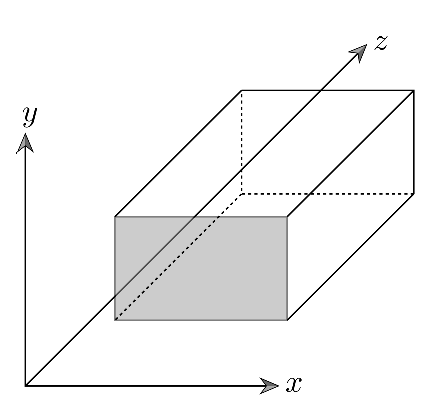
\includegraphics[width=0.33\linewidth]{chap06/Orthoviewingvolume.eps}
    \caption{正交视见体是相机空间中的轴对齐框,
        其定义使该区域内的物体投影到该框$z=\text{near}$的一面上。}
    \label{fig:6.2}
\end{figure}

\reffig{6.3}比较了用正交投影和下节定义的透视投影来渲染的结果
\sidenote{译者注:原图为exr格式,此处转换为png格式以便制作插图,
    图像细节和色域可能发生细微变化。后续均作此处理,读者可到原书官网查看原图。}。
\begin{figure}[htbp]
    \centering
    \subfloat[正交]{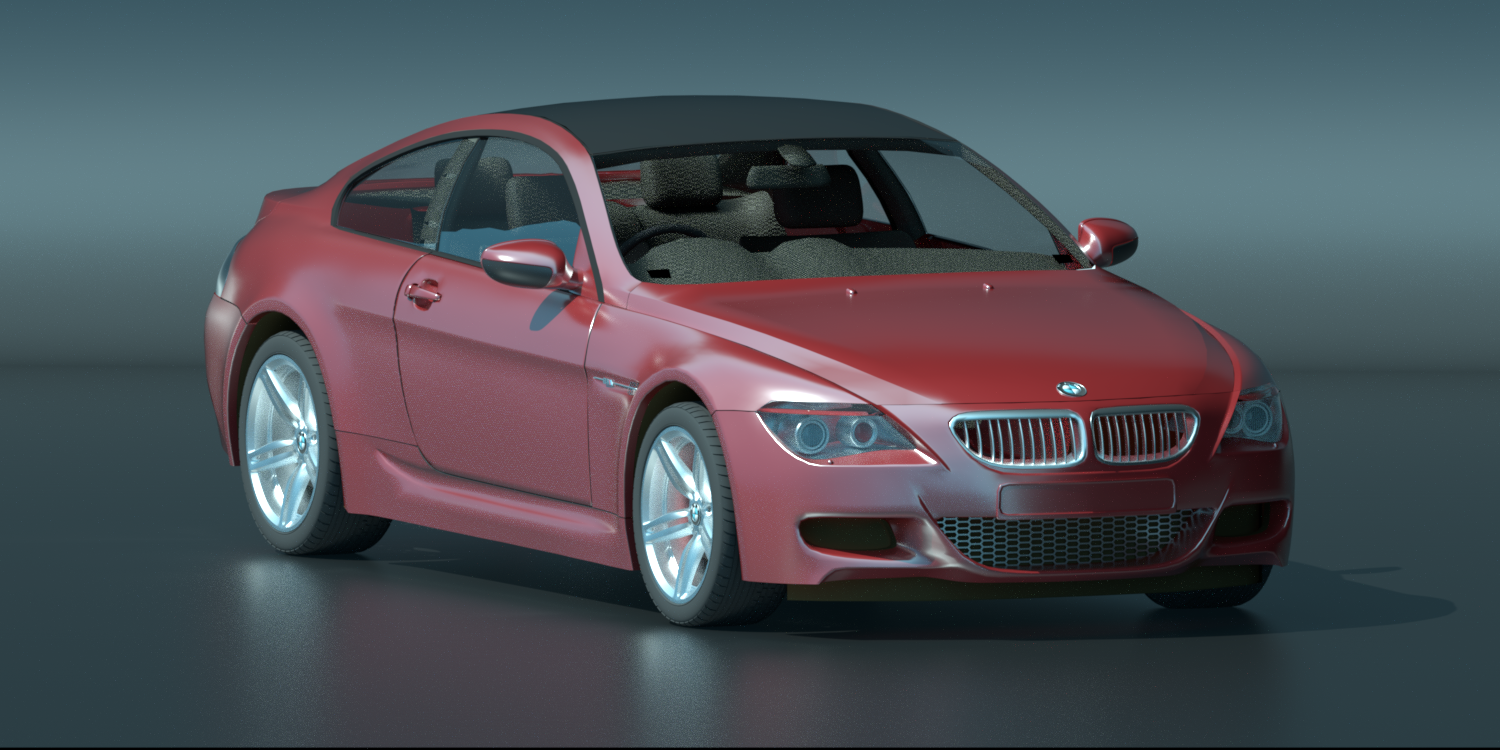
\includegraphics[width=\linewidth]{chap06/car-ortho.png}\label{fig:6.3.1}}\\
    \subfloat[透视]{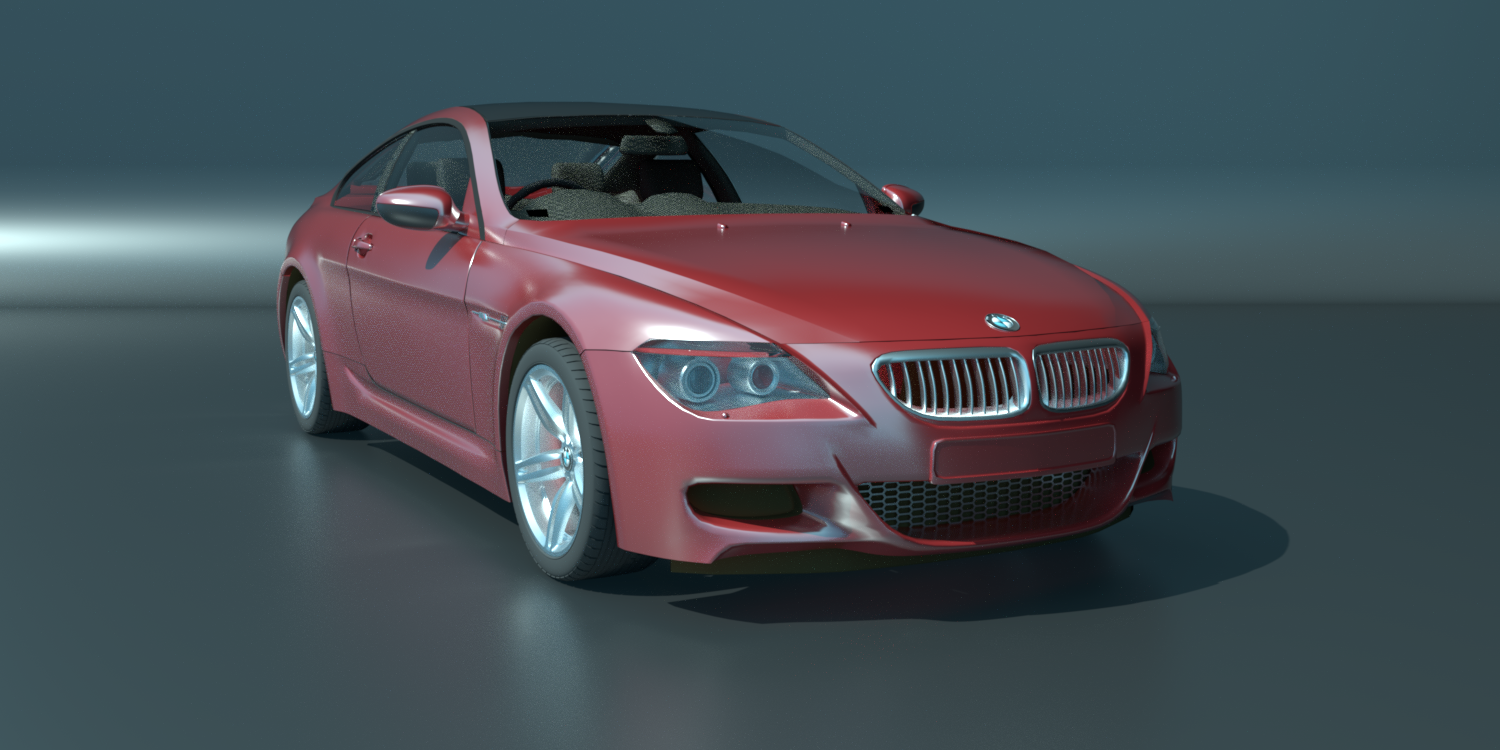
\includegraphics[width=\linewidth]{chap06/car-perspective.png}\label{fig:6.3.2}}
    \caption{用不同相机模型渲染的汽车模型。用(a)正交和(b)透视相机从同一视点渲染汽车。
        缺少前缩使得正交视角看起来深度更少,但它保留了平行线,是很有用的特性。}
    \label{fig:6.3}
\end{figure}

正交相机构造函数用稍后定义的函数\refvar{Orthographic}{()}生成正交变换矩阵。
\begin{lstlisting}
`\initcode{OrthographicCamera Public Methods}{=}`
`\refvar{OrthographicCamera}{}`(const `\refvar{AnimatedTransform}{}` &CameraToWorld,
        const `\refvar{Bounds2f}{}` &screenWindow, `\refvar{Float}{}` shutterOpen,
        `\refvar{Float}{}` shutterClose, `\refvar{Float}{}` lensRadius, `\refvar{Float}{}` focalDistance,
        `\refvar{Film}{}` *film, const `\refvar{Medium}{}` *medium)
    : `\refvar{ProjectiveCamera}{}`(CameraToWorld, `\refvar{Orthographic}{}`(0, 1),
                       screenWindow, shutterOpen, shutterClose,
                       lensRadius, focalDistance, film, medium) {
    `\refcode{Compute differential changes in origin for orthographic camera rays}{}`
}
\end{lstlisting}

正交视角变换保持$x$和$y$坐标不变但将近处平面的$z$值映射为0而远处平面的$z$值映射为1。
为此,场景先沿$z$轴平移使得近处平面对齐到$z=0$。
然后,场景按$z$缩放使得远处平面映射为$z=1$。
这两个变换合成得到整个变换。(对于像pbrt那样的光线追踪器,
我们想让近处平面位于0处,这样光线就会从穿过相机位置的平面上发出;
远处平面偏移量不是很重要。)
\begin{lstlisting}
`\refcode{Transform Method Definitions}{+=}\lastnext{TransformMethodDefinitions}`
`\refvar{Transform}{}` `\initvar{Orthographic}{}`(`\refvar{Float}{}` zNear, `\refvar{Float}{}` zFar) {
    return `\refvar{Scale}{}`(1, 1, 1 / (zFar - zNear)) *
           `\refvar{Translate}{}`(`\refvar{Vector3f}{}`(0, 0, -zNear));
}
\end{lstlisting}

幸亏正交投影很简单,在方法\refvar[OrthographicCamera::GenerateRayDifferential]{GenerateRayDifferential}{()}中
很容易直接计算$x$和$y$方向的差分射线。
差分射线的方向将和主射线一样(它们对于一个正交相机生成的所有光线都是这样),
且端点差异对于所有射线也会一样。
因此,这里的构造函数预先计算射线端点因胶片平面上在$x$和$y$方向移动单个像素而
在相机空间坐标中移动了多少。
\begin{lstlisting}
`\initcode{Compute differential changes in origin for orthographic camera rays}{=}`
`\refvar[OrthographicCamera::dxCamera]{dxCamera}{}` = `\refvar{RasterToCamera}{}`(`\refvar{Vector3f}{}`(1, 0, 0));
`\refvar[OrthographicCamera::dyCamera]{dyCamera}{}` = `\refvar{RasterToCamera}{}`(`\refvar{Vector3f}{}`(0, 1, 0));
\end{lstlisting}
\begin{lstlisting}
`\initcode{OrthographicCamera Private Data}{=}`
`\refvar{Vector3f}{}` `\initvar[OrthographicCamera::dxCamera]{dxCamera}{}`, `\initvar[OrthographicCamera::dyCamera]{dyCamera}{}`;
\end{lstlisting}

我们现在可以执行代码取栅格空间中的一个样本点并将其变为相机光线。
\reffig{6.4}总结了该过程。首先,栅格空间样本位置变换为相机空间的一点,
即给出近处平面上一点作为相机光线的端点。
因为相机空间观察方向沿$z$轴指出,相机空间光线方向为$(0,0,1)$。

\begin{figure}[htbp]
    \centering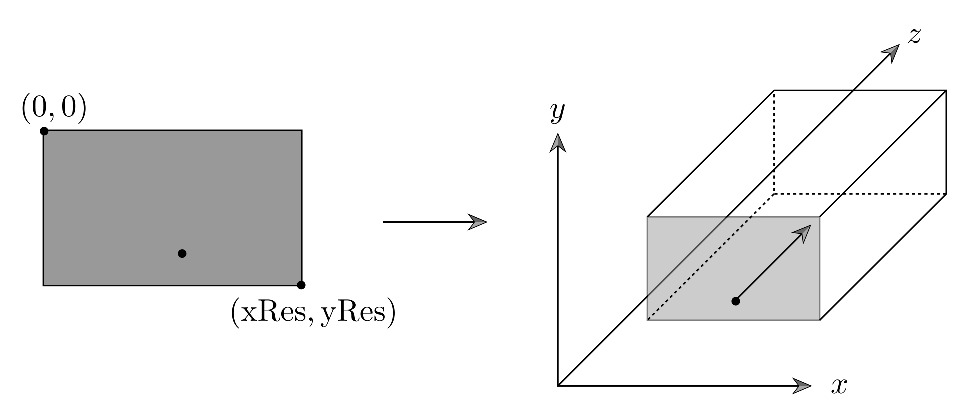
\includegraphics[width=0.8\linewidth]{chap06/Orthogenerateray.eps}
    \caption{为了用正交相机创建光线,胶片平面上的栅格空间位置被变换到相机空间,
        给出近处平面上的射线端点。相机空间中光线的方向为$(0,0,1)$,沿$z$轴。}
    \label{fig:6.4}
\end{figure}

若为该场景启用景深,则修改射线端点和方向来模拟景深。本节将稍后解释景深。
光线的时间值通过按偏移量\refvar{CameraSample::time}{}(在范围$[0,1)$内)
在快门开启和关闭间线性插值来设置。最后,光线在被返回前变换到世界空间。
\begin{lstlisting}
`\initcode{OrthographicCamera Definitions}{=}\initnext{OrthographicCameraDefinitions}`
`\refvar{Float}{}` `\refvar{OrthographicCamera}{}`::`\initvar[OrthographicCamera::GenerateRay]{\refvar{GenerateRay}{}}{}`(const `\refvar{CameraSample}{}` &sample,
        `\refvar{Ray}{}` *ray) const {
    `\refcode{Compute raster and camera sample positions}{}`
    *ray = `\refvar{Ray}{}`(pCamera, `\refvar{Vector3f}{}`(0, 0, 1));
    `\refcode{Modify ray for depth of field}{}`
    ray->`\refvar[Ray::time]{time}{}` = `\refvar{Lerp}{}`(sample.`\refvar[CameraSample::time]{time}{}`, `\refvar{shutterOpen}{}`, `\refvar{shutterClose}{}`);
    ray->`\refvar[Ray::medium]{medium}{}` = `\refvar[Camera::medium]{medium}{}`;
    *ray = `\refvar{CameraToWorld}{}`(*ray);
    return 1;
}
\end{lstlisting}

一旦设置好所有变换矩阵,就很容易将栅格空间样本变换到相机空间。
\begin{lstlisting}
`\initcode{Compute raster and camera sample positions}{=}`
`\refvar{Point3f}{}` pFilm = `\refvar{Point3f}{}`(sample.`\refvar{pFilm}{}`.x, sample.`\refvar{pFilm}{}`.y, 0);
`\refvar{Point3f}{}` pCamera = `\refvar{RasterToCamera}{}`(pFilm);
\end{lstlisting}

\refvar[OrthographicCamera::GenerateRayDifferential]{GenerateRayDifferential}{()}的实现执行一样的计算来生成相机主光线。
差分射线端点用在\refvar{OrthographicCamera}{}构造函数中算得的偏移量求出,
然后将整个射线差分变换到世界空间。
\begin{lstlisting}
`\refcode{OrthographicCamera Definitions}{+=}\lastcode{OrthographicCameraDefinitions}`
`\refvar{Float}{}` `\refvar{OrthographicCamera}{}`::`\initvar[OrthographicCamera::GenerateRayDifferential]{\refvar{GenerateRayDifferential}{}}{}`(
        const `\refvar{CameraSample}{}` &sample, `\refvar{RayDifferential}{}` *ray) const {
    `\refcode{Compute main orthographic viewing ray}{}`
    `\refcode{Compute ray differentials for OrthographicCamera}{}`
    ray->`\refvar[Ray::time]{time}{}` = `\refvar{Lerp}{}`(sample.`\refvar[CameraSample::time]{time}{}`, `\refvar{shutterOpen}{}`, `\refvar{shutterClose}{}`);
    ray->`\refvar{hasDifferentials}{}` = true;
    ray->`\refvar[Ray::medium]{medium}{}` = `\refvar[Camera::medium]{medium}{}`;
    *ray = `\refvar{CameraToWorld}{}`(*ray);
    return 1;
}
\end{lstlisting}
\begin{lstlisting}
`\initcode{Compute main orthographic viewing ray}{=}`
`\refcode{Compute raster and camera sample positions}{}`
*ray = `\refvar{RayDifferential}{}`(pCamera, `\refvar{Vector3f}{}`(0, 0, 1));
`\refcode{Modify ray for depth of field}{}`
\end{lstlisting}
\begin{lstlisting}
`\initcode{Compute ray differentials for OrthographicCamera}{=}`
if (`\refvar{lensRadius}{}` > 0) {
    `\refcode{Compute OrthographicCamera ray differentials accounting for lens}{}`
} else {
    ray->`\refvar{rxOrigin}{}` = ray->`\refvar[Ray::o]{o}{}` + `\refvar[OrthographicCamera::dxCamera]{dxCamera}{}`;
    ray->`\refvar{ryOrigin}{}` = ray->`\refvar[Ray::o]{o}{}` + `\refvar[OrthographicCamera::dyCamera]{dyCamera}{}`;
    ray->`\refvar{rxDirection}{}` = ray->`\refvar{ryDirection}{}` = ray->`\refvar[Ray::d]{d}{}`;
}
\end{lstlisting}
\begin{lstlisting}
`\initcode{Compute OrthographicCamera ray differentials accounting for lens}{=}`
`\refcode{Sample point on lens}{}`
`\refvar{Float}{}` ft = focalDistance / ray->`\refvar[Ray::d]{d}{}`.z;

`\refvar{Point3f}{}` pFocus = pCamera + `\refvar[OrthographicCamera::dxCamera]{dxCamera}{}` + (ft * `\refvar{Vector3f}{}`(0, 0, 1));
ray->`\refvar{rxOrigin}{}` = `\refvar{Point3f}{}`(pLens.x, pLens.y, 0);
ray->`\refvar{rxDirection}{}` = `\refvar{Normalize}{}`(pFocus - ray->`\refvar{rxOrigin}{}`);

pFocus = pCamera + `\refvar[OrthographicCamera::dyCamera]{dyCamera}{}` + (ft * `\refvar{Vector3f}{}`(0, 0, 1));
ray->`\refvar{ryOrigin}{}` = `\refvar{Point3f}{}`(pLens.x, pLens.y, 0);
ray->`\refvar{ryDirection}{}` = `\refvar{Normalize}{}`(pFocus - ray->`\refvar{ryOrigin}{}`);
\end{lstlisting}

\subsection{透视相机}\label{sub:透视相机}
透视投影和正交投影相似,也把一个空间体投影到2D胶片平面上。
然而,它包含前缩效应:远处物体比近处相同尺寸的物体投影得更小。
不像正交投影那样,透视投影不保持距离和角度,平行线也不再保持平行。
透视投影非常符合眼睛或相机透镜生成3D世界图像的方式。
投影相机实现于文件\href{https://github.com/mmp/pbrt-v3/blob/master/src/cameras/perspective.h}{\ttfamily cameras/perspective.h}
和\href{https://github.com/mmp/pbrt-v3/blob/master/src/cameras/perspective.cpp}{\ttfamily cameras/perspective.cpp}中。
\begin{lstlisting}
`\initcode{PerspectiveCamera Declarations}{=}`
class `\initvar{PerspectiveCamera}{}` : public `\refvar{ProjectiveCamera}{}` {
public:
    `\refcode{PerspectiveCamera Public Methods}{}`
private:
    `\refcode{PerspectiveCamera Private Data}{}`
};
\end{lstlisting}
\begin{lstlisting}
`\initcode{PerspectiveCamera Method Definitions}{=}\initnext{PerspectiveCameraMethodDefinitions}`
`\refvar{PerspectiveCamera}{}`::`\refvar{PerspectiveCamera}{}`(
        const `\refvar{AnimatedTransform}{}` &CameraToWorld,
        const `\refvar{Bounds2f}{}` &screenWindow, `\refvar{Float}{}` shutterOpen,
        `\refvar{Float}{}` shutterClose, `\refvar{Float}{}` lensRadius, `\refvar{Float}{}` focalDistance,
        `\refvar{Float}{}` fov, `\refvar{Film}{}` *film, const `\refvar{Medium}{}` *medium)
    : `\refvar{ProjectiveCamera}{}`(CameraToWorld, `\refvar{Perspective}{}`(fov, 1e-2f, 1000.f),
                       screenWindow, shutterOpen, shutterClose,
                       lensRadius, focalDistance, film, medium) {
    `\refcode{Compute differential changes in origin for perspective camera rays}{}`
    `\refcode{Compute image plane bounds at z=1 for PerspectiveCamera}{}`
}
\end{lstlisting}

透视投影描述了场景的透视图。
场景中的点投影到垂直于$z$轴的视平面上。
函数\refvar{Perspective}{()}计算该变换;
它接收视场角度{\ttfamily fov}以及到近处$z$平面和远处$z$平面的距离。
在透视投影后,近处$z$平面上的点映射为$z=0$,远处平面上的点则有$z=1$(\reffig{6.5})。
对于基于栅格化的渲染系统,仔细设置这些平面的位置很重要;
它们决定了要渲染的场景的$z$范围,但将它们取值的量级设置得相差过大可能导致数值精度误差。
对于像pbrt的光线追踪器,可以按其位置任意设置它们。
\begin{figure}[htbp]
    \centering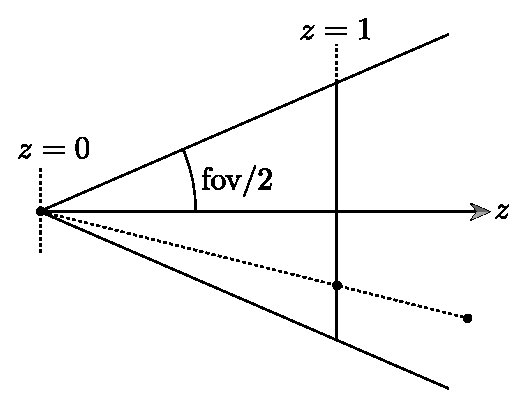
\includegraphics[width=0.5\linewidth]{chap06/Perspectivetransformationmatrix.eps}
    \caption{投影变换矩阵将相机空间里的点投影到胶片平面。
        被投影点的$x'$和$y'$坐标等于投影前$x$和$y$坐标除以$z$坐标。
        投影后的$z'$坐标的计算使得近处平面的点映射为$z'=0$而
        远处平面的点映射为$z'=1$。}
    \label{fig:6.5}
\end{figure}

\begin{lstlisting}
`\refcode{Transform Method Definitions}{+=}\lastcode{TransformMethodDefinitions}`
`\refvar{Transform}{}` `\initvar{Perspective}{}`(`\refvar{Float}{}` fov, `\refvar{Float}{}` n, `\refvar{Float}{}` f) {
    `\refcode{Perform projective divide for perspective projection}{}`
    `\refcode{Scale canonical perspective view to specified field of view}{}`
}
\end{lstlisting}
该变换最容易理解,分两个步骤:
\begin{enumerate}
    \item 相机空间的点$\bm p$被投影到视平面上。
          一点代数计算证明视平面上投影后的$x'$和$y'$坐标可计算为$x$和$y$除以点的$z$坐标值。
          投影后的深度$z$被重新映射使近处平面的$z$值为0而远处平面的$z$值为1。
          我们要做的计算为
          \begin{align*}
              x' & =\frac{x}{z}\, ,           \\
              y' & =\frac{y}{z}\, ,           \\
              z' & =\frac{f(z-n)}{z(f-n)}\, .
          \end{align*}
          整个该计算可用齐次坐标编码为$4\times4$矩阵:
          \begin{align*}
              \left[\begin{array}{cccc}
                      1 & 0 & 0             & 0               \\
                      0 & 1 & 0             & 0               \\
                      0 & 0 & \frac{f}{f-n} & -\frac{fn}{f-n} \\
                      0 & 0 & 1             & 0
                  \end{array}\right]
          \end{align*}
          \begin{lstlisting}
`\initcode{Perform projective divide for perspective projection}{=}`
`\refvar{Matrix4x4}{}` persp(1, 0,           0,              0,
                0, 1,           0,              0,
                0, 0, f / (f - n), -f*n / (f - n),
                0, 0,           1,              0);
\end{lstlisting}
    \item 用户指定的视场角({\ttfamily fov})通过缩放投影平面上的$(x,y)$值
          使得视场内的点投影到视平面上坐标$[-1,1]$内来实现。
          对于正方形图像,屏幕空间内$x$和$y$都在$[-1,1]$内。
          否则,图像更窄的那个方向映射到$[-1,1]$,
          更宽的方向映射到成比例的更大屏幕空间值范围。
          回想正切等于直角三角形对边与邻边之比。
          这里邻边长为1,所以对边长为$\tan\frac{\text{\ttfamily fov}}{2}$。
          用该长度倒数缩放将视场映射到$[-1,1]$内的范围。
\end{enumerate}
\begin{lstlisting}
`\initcode{Scale canonical perspective view to specified field of view}{=}`
`\refvar{Float}{}` invTanAng = 1 / std::tan(`\refvar{Radians}{}`(fov) / 2);
return `\refvar{Scale}{}`(invTanAng, invTanAng, 1) * `\refvar{Transform}{}`(persp);
\end{lstlisting}

类似于\refvar{OrthographicCamera}{},关于\refvar{PerspectiveCamera}{}生成的
相机光线如何随着我们移动胶片平面上的像素而改变的信息可在构造函数中预先算出。
这里我们计算相机空间近处投影平面上的位置随像素位置移动而发生的变化。
\begin{lstlisting}
`\initcode{Compute differential changes in origin for perspective camera rays}{=}`
`\refvar[PerspectiveCamera::dxCamera]{dxCamera}{}` = (`\refvar{RasterToCamera}{}`(`\refvar{Point3f}{}`(1, 0, 0)) -
            `\refvar{RasterToCamera}{}`(`\refvar{Point3f}{}`(0, 0, 0)));
`\refvar[PerspectiveCamera::dyCamera]{dyCamera}{}` = (`\refvar{RasterToCamera}{}`(`\refvar{Point3f}{}`(0, 1, 0)) -
            `\refvar{RasterToCamera}{}`(`\refvar{Point3f}{}`(0, 0, 0)));
\end{lstlisting}
\begin{lstlisting}
`\initcode{PerspectiveCamera Private Data}{=}\initnext{PerspectiveCameraPrivateData}`
`\refvar{Vector3f}{}` `\initvar[PerspectiveCamera::dxCamera]{dxCamera}{}`, `\initvar[PerspectiveCamera::dyCamera]{dyCamera}{}`;
\end{lstlisting}

用透视投影时,所有光线都从相机空间原点$(0,0,0)$发出。
光线的方向由从原点指向近处平面上的点{\ttfamily pCamera}的向量给出,
该点对应提供的\refvar{CameraSample}{}的{\ttfamily pFilm}位置。
换句话说,该光线方向向量的每个分量等于该点的位置,
所以不需做无用减法来计算该方向,我们只需直接用点{\ttfamily pCamera}来初始化该方向。
\begin{lstlisting}
`\refcode{PerspectiveCamera Method Definitions}{+=}\lastnext{PerspectiveCameraMethodDefinitions}`
`\refvar{Float}{}` `\refvar{PerspectiveCamera}{}`::`\initvar[PerspectiveCamera::GenerateRay]{\refvar{GenerateRay}{}}{}`(const `\refvar{CameraSample}{}` &sample,
        `\refvar{Ray}{}` *ray) const {
    `\refcode{Compute raster and camera sample positions}{}`
    *ray = `\refvar{Ray}{}`(`\refvar{Point3f}{}`(0, 0, 0), `\refvar{Normalize}{}`(`\refvar{Vector3f}{}`(pCamera)));
    `\refcode{Modify ray for depth of field}{}`
    ray->`\refvar[Ray::time]{time}{}` = `\refvar{Lerp}{}`(sample.`\refvar[CameraSample::time]{time}{}`, `\refvar{shutterOpen}{}`, `\refvar{shutterClose}{}`);
    ray->`\refvar[Ray::medium]{medium}{}` = `\refvar[Camera::medium]{medium}{}`;
    *ray = `\refvar{CameraToWorld}{}`(*ray);
    return 1;
}
\end{lstlisting}

方法\refvar[PerspectiveCamera::GenerateRayDifferential]{GenerateRayDifferential}{()}遵
循\refvar[PerspectiveCamera::GenerateRay]{GenerateRay}{()}的实现,只是多了计算差分射线的代码片。
\begin{lstlisting}
`\initcode{PerspectiveCamera Public Methods}{=}`
`\refvar{Float}{}` `\initvar[PerspectiveCamera::GenerateRayDifferential]{\refvar{GenerateRayDifferential}{}}{}`(const `\refvar{CameraSample}{}` &sample,
                              `\refvar{RayDifferential}{}` *ray) const;
\end{lstlisting}
\begin{lstlisting}
`\initcode{Compute offset rays for PerspectiveCamera ray differentials}{=}`
if (lensRadius > 0) {
    `\refcode{Compute PerspectiveCamera ray differentials accounting for lens}{}`
} else {
    ray->`\refvar{rxOrigin}{}` = ray->`\refvar{ryOrigin}{}` = ray->`\refvar[Ray::o]{o}{}`;
    ray->`\refvar{rxDirection}{}` = `\refvar{Normalize}{}`(`\refvar{Vector3f}{}`(pCamera) + `\refvar[PerspectiveCamera::dxCamera]{dxCamera}{}`);
    ray->`\refvar{ryDirection}{}` = `\refvar{Normalize}{}`(`\refvar{Vector3f}{}`(pCamera) + `\refvar[PerspectiveCamera::dyCamera]{dyCamera}{}`);
}
\end{lstlisting}
\begin{lstlisting}
`\initcode{Compute PerspectiveCamera ray differentials accounting for lens}{=}`
`\refcode{Sample point on lens}{}`
`\refvar{Vector3f}{}` dx = `\refvar{Normalize}{}`(`\refvar{Vector3f}{}`(pCamera + `\refvar[PerspectiveCamera::dxCamera]{dxCamera}{}`));
`\refvar{Float}{}` ft = focalDistance / dx.z;
`\refvar{Point3f}{}` pFocus = `\refvar{Point3f}{}`(0, 0, 0) + (ft * dx);
ray->`\refvar{rxOrigin}{}` = `\refvar{Point3f}{}`(pLens.x, pLens.y, 0);
ray->`\refvar{rxDirection}{}` = `\refvar{Normalize}{}`(pFocus - ray->`\refvar{rxOrigin}{}`);

`\refvar{Vector3f}{}` dy = `\refvar{Normalize}{}`(`\refvar{Vector3f}{}`(pCamera + `\refvar[PerspectiveCamera::dyCamera]{dyCamera}{}`));
ft = focalDistance / dy.z;
pFocus = `\refvar{Point3f}{}`(0, 0, 0) + (ft * dy);
ray->`\refvar{ryOrigin}{}` = `\refvar{Point3f}{}`(pLens.x, pLens.y, 0);
ray->`\refvar{ryDirection}{}` = `\refvar{Normalize}{}`(pFocus - ray->`\refvar{ryOrigin}{}`);
\end{lstlisting}

\subsection{薄透镜模型与景深}\label{sub:薄透镜模型与景深}
只允许光线穿过单个点后到达胶片的理想针孔相机是不可物理实现的;
尽管可以用具有极小\keyindex{光圈}{aperture}{}的相机近似该情况,但小光圈只允许相对很少的光到达胶片传感器。
用小光圈时需要较长曝光时间来捕获足够的光子以准确获取图像,
这反过来会导致场景中在相机快门开启时正运动的物体变模糊。

真实相机具有透镜系统,它将光聚焦穿过大小有限的光圈后打到胶片平面上。
相机设计者(以及使用可调光圈相机的摄影师)面临权衡:
光圈越大,到达胶片的光越多,需要的曝光越短。
然而,透镜只能聚焦于单个平面(\keyindex{焦平面}{focal plane}{}),
场景中的物体离该平面越远就越模糊。
光圈越大,该效应就越显著:处在与透镜系统聚焦深度不同处的物体变得越发模糊。

\refsec{逼真相机}的相机模型对真实相机中的透镜系统实现了相当准确的模拟。
对于目前介绍的简单相机模型,我们可以运用光学中的经典近似,\keyindex{薄透镜近似}{thin lens approximation}{},
借助传统计算机图形学投影模型来对有限光圈的效应建模。
薄透镜近似将光学系统建模为球形剖面的单个透镜,
该透镜的厚度相比于透镜的\keyindex{曲率半径}{radius of curvature}{}很小
(\refsub{厚透镜近似}介绍更一般的厚透镜近似,它假设透镜的厚度是不可忽略的)。

在薄透镜近似下,平行于\keyindex{光轴}{optical axis}{}的入射光线穿过透镜后
聚在透镜后方称为\keyindex{焦点}{focal point}{}的点上。
若胶片平面置于透镜后方距离等于\keyindex{焦距}{focal length}{}的地方,
则无限远的物体将对好焦,它们成像为胶片上的单个点。

\reffig{6.6}展示了基本设置。这里我们遵循典型透镜坐标系统的惯例
让透镜垂直于$z$轴并位于$z=0$,场景在$-z$
(注意这个坐标系统和我们给相机空间用的看向$+z$的不同)。
透镜场景一侧的距离记为无撇的变量$z$,透镜胶片一侧的距离(正的$z$)记为有撇的$z'$。
\begin{figure}[htbp]
    \centering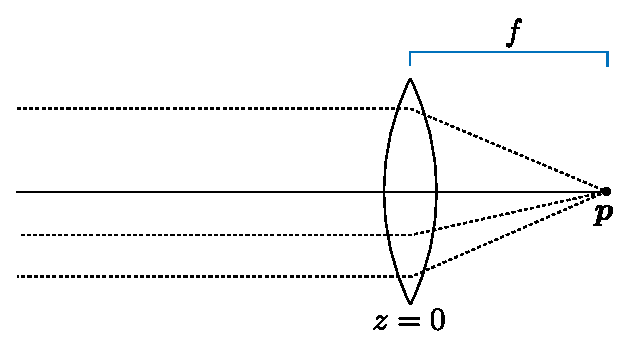
\includegraphics[width=0.6\linewidth]{chap06/Thinlens.eps}
    \caption{沿$z$轴置于$z=0$处的薄透镜。平行于光轴的入射光线穿过薄透镜后(虚线)
        均通过点$\bm p$,即焦点。透镜与焦点的距离$f$为透镜的焦距。}
    \label{fig:6.6}
\end{figure}

对于场景中与焦距为$f$的薄透镜距离为$z$的点,
\keyindex{高斯透镜方程}{Gaussian lens equation}{}将
物体与透镜的距离和透镜与像点的距离联系起来:
\begin{align}\label{eq:6.1}
    \frac{1}{z'}-\frac{1}{z}=\frac{1}{f}\, .
\end{align}
注意对于$z=-\infty$,正如预期那样我们有$z'=f$。

我们可以用高斯透镜方程求解透镜与胶片的距离即\keyindex{对焦距离}{focal distance}{}
\sidenote{译者注:此处“focal distance”译为“对焦距离”是折中做法,
    笔者查阅到的一些资料中“对焦距离”的含义与这里书中的有所不同,
    故目前还不确定该词组的正确翻译。欢迎读者提供帮助。}
来为某个$z$设置焦平面(\reffig{6.7}):
\begin{align}\label{eq:6.2}
    z'=\frac{fz}{f+z}\, .
\end{align}

\begin{figure}[htbp]
    \centering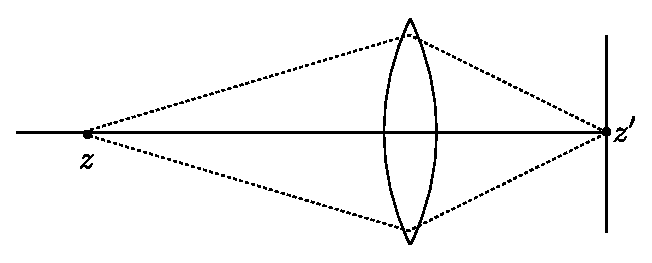
\includegraphics[width=0.6\linewidth]{chap06/Focusthinlens.eps}
    \caption{为了让薄透镜聚焦场景中的深度$z$处,
        \refeq{6.2}可用于计算$z$处的点聚焦到的透镜胶片一侧的距离$z'$。
        通过调整透镜和胶片平面的距离执行对焦。}
    \label{fig:6.7}
\end{figure}

不在焦平面上的点在胶片平面上成像为圆斑,而不是单个点。
该斑的边界称为\keyindex{弥散圆}{circle of confusion}{}。
弥散圆的大小受到光线穿过的光圈\keyindex{直径}{diameter}{}、
对焦距离以及物体与透镜间距离的影响。
\reffig{6.8}展示了具有一系列龙模型副本的场景中的这种效应,即景深。
随着透镜光圈尺寸增大,离焦平面越远的点模糊度越大。
注意在所有图像中从右边数第二个龙都保持对准焦,
因为焦平面就放置在其深度处。
\begin{figure}[htbp]
    \centering
    \subfloat[无景深]{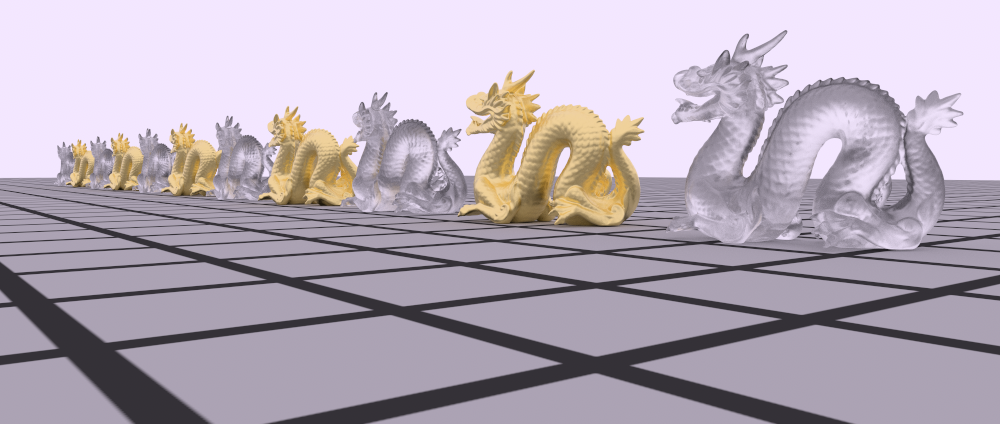
\includegraphics[width=0.85\linewidth]{chap06/dragons-nodof.png}\label{fig:6.8.1}}\\
    \subfloat[小光圈]{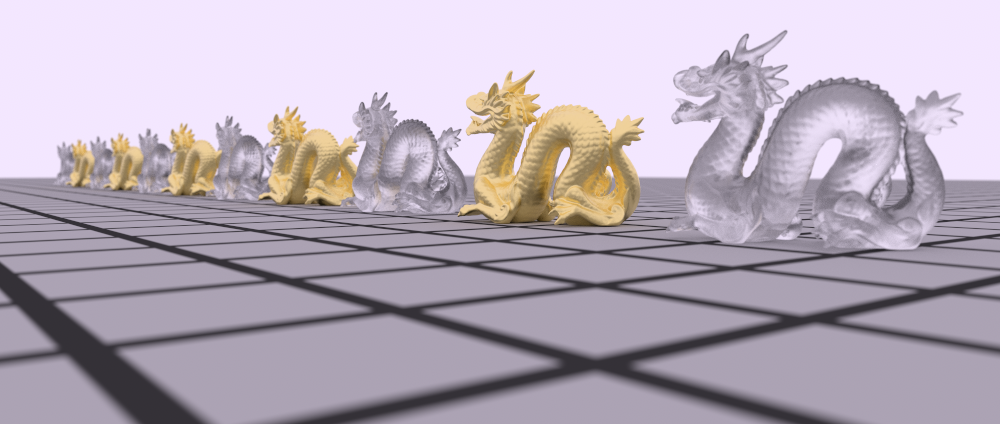
\includegraphics[width=0.85\linewidth]{chap06/dragons-small-dof.png}\label{fig:6.8.2}}\\
    \subfloat[中光圈]{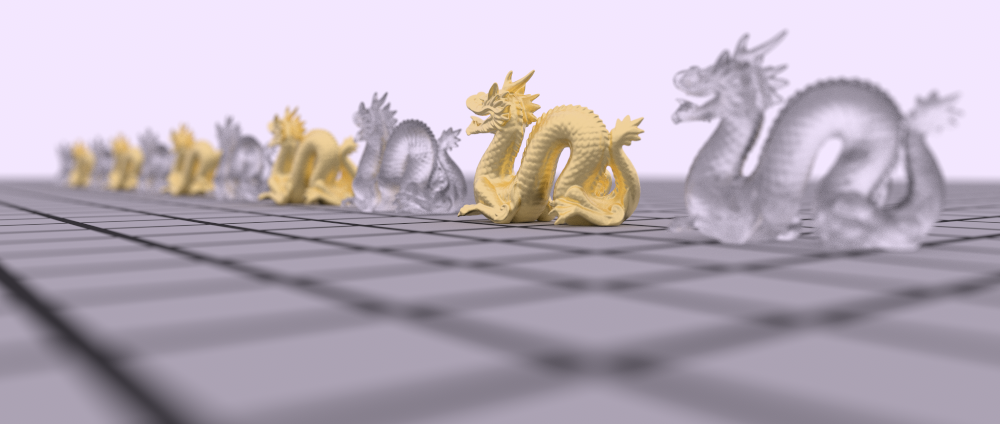
\includegraphics[width=0.85\linewidth]{chap06/dragons-med-dof.png}\label{fig:6.8.3}}\\
    \subfloat[大光圈]{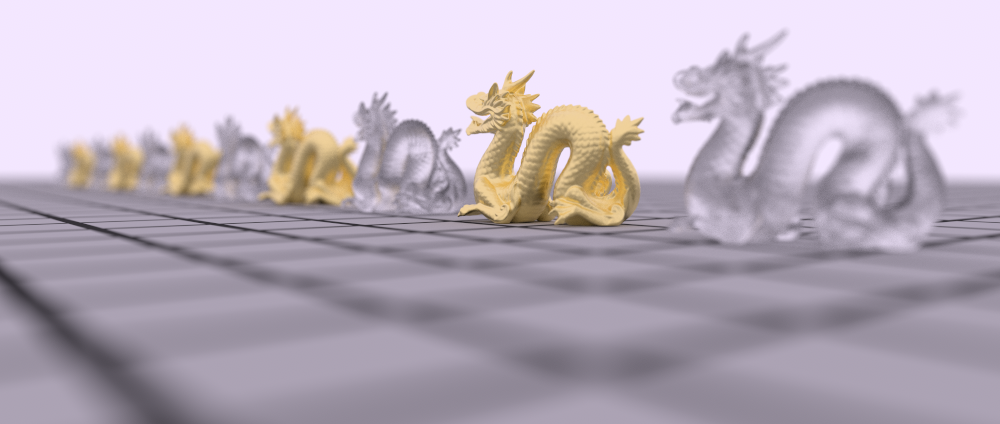
\includegraphics[width=0.85\linewidth]{chap06/dragons-large-dof.png}\label{fig:6.8.4}}
    \caption{(1)无景深渲染场景,(2)相对较小透镜光圈导致的景深,让失焦区域只有少量模糊,
    (3)和(4)中随着透镜光圈尺寸增大,失焦区域弥散圆的尺寸也增大,使胶片平面上的模糊程度更大。}
    \label{fig:6.8}
\end{figure}

\reffig{6.9}展示了用于渲染景观场景的景深。
注意该效应是如何把观察者的视线吸引到图像中间对焦的小草上的。
\begin{figure}[htbp]
    \centering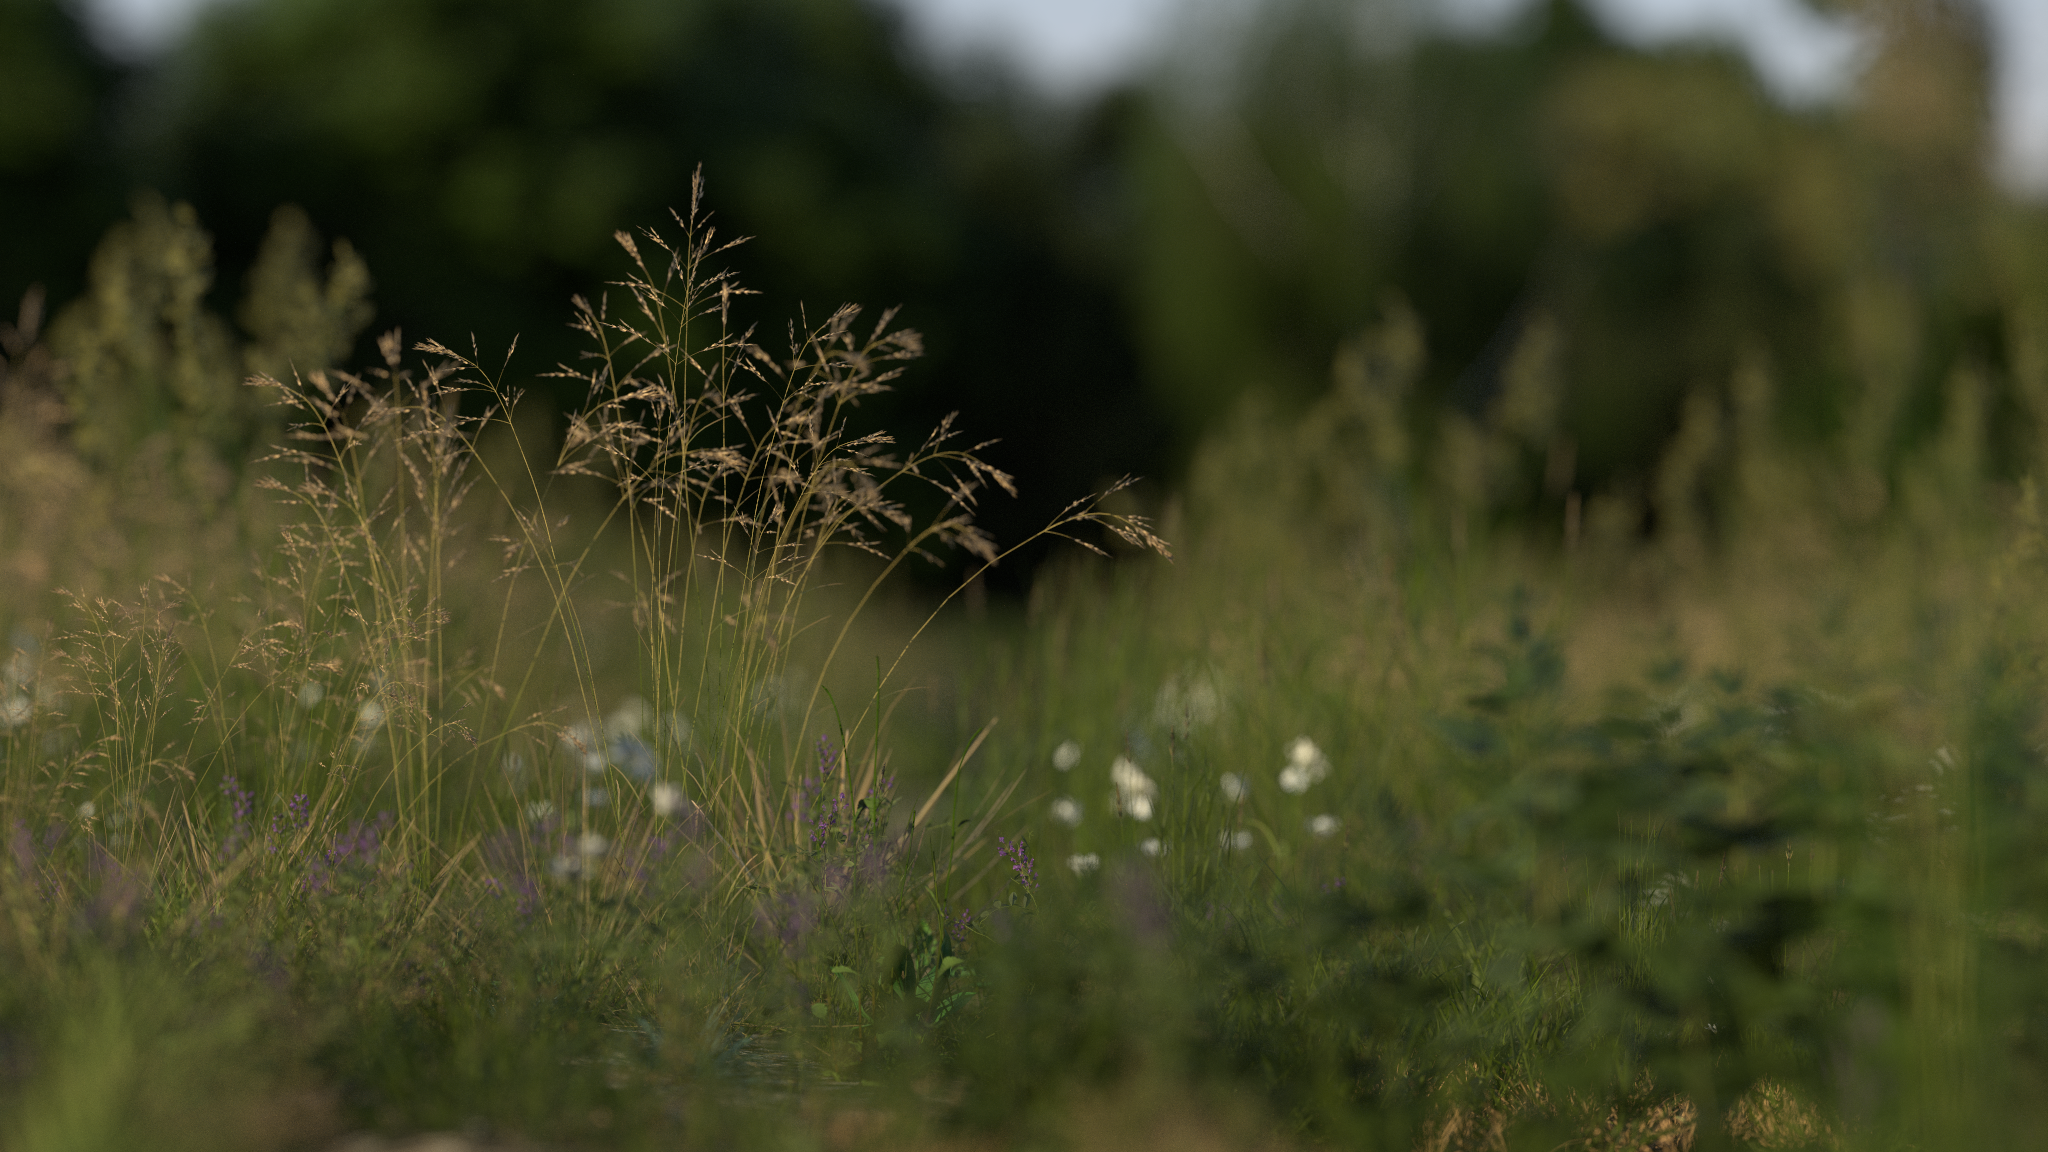
\includegraphics[width=\linewidth]{chap06/landscape-dof.png}
    \caption{景深赋予这部分景观场景很强的纵深感({\itshape 感谢Laubwerk提供场景})。}
    \label{fig:6.9}
\end{figure}

实践中,